\documentclass{beamer}
\usepackage{beamerthemeshadow}
\usepackage[spanish]{babel}
\usepackage[utf8]{inputenc}
\usepackage[T1]{fontenc}
\usepackage{enumerate}
\usepackage{mathtools}
\usepackage{mathpazo}
\usepackage{amssymb}
\usepackage{stmaryrd}
\usepackage{lmodern}

%\setbeamertemplate{theorems}[ams style] % numbered
\theoremstyle{definition}
\makeatletter
\setbeamertemplate{theorem begin}
{%
  \inserttheoremheadfont \bfseries
  \inserttheoremname \inserttheoremnumber
  \ifx\inserttheoremaddition\@empty\else\ (\inserttheoremaddition)\fi%
  :
  \normalfont
}
\setbeamertemplate{theorem end}{%
  % empty
}
\makeatother


\begin{document}
\title{Compresión: JPEG}
\author{Gabriel Thibeault y Gonzalo Ciruelos}
\date{13 de diciembre de 2017}


%\frame{\titlepage}

\section{Introducción}
\frame{\frametitle{El trabajo}

Este trabajo se basa en la realización de una implementación del algoritmo
de compresión usado por el estándar de JPEG.

\hspace{1cm}

JPEG es un método común de compresión con pérdida para imágenes digitales.
El grado de compresión puede ajustarse, permitiendo un compromiso entre
tamaño y calidad de la imágen resultante.

\hspace{2cm}

El trabajo en el cual basamos nuestra implementación es

\begin{center}
  Gregory K. Wallace. The JPEG still picture compression standard.
  \emph{IEEE Transactions on Consumer Electronics}, 38(1):XVIII--XXXIV, 1992.
\end{center}
}


\frame{\frametitle{Codificación de Huffman}

\begin{enumerate}
  \item Diferencial de $DC$s.
  \item Representación zig-zag.
  \item Run lenghts.
  \item Codificación de Huffman usando esos pares como los símbolos del lenguaje.
\end{enumerate}

\begin{center}
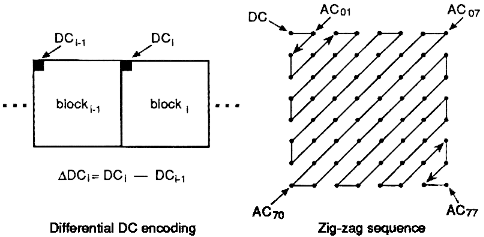
\includegraphics[width=5cm]{images/huffman.png}
\end{center}

\[
  [10, 1, 1, 0, 0, 0, 0, 2, 1, 0, 0, 1, 0, 0, 0, 0]
\]
\[
  \to [(0, 10), (0, 1), (0, 1), (4, 2), (0, 1), (2, 1)]
\]
}

\frame{
\huge
\begin{center}
¿Preguntas?
\end{center}
}

\end{document}


